\documentclass[12pt]{article}
   
\usepackage[utf8]{inputenc}
   \usepackage{graphicx}
   \usepackage{appendix}
   \usepackage{float}
   \usepackage{subcaption}
   %\usepackage{mathtools}
   \usepackage{amsmath}
   \usepackage{hyperref}
\hypersetup{
    colorlinks=true,
    linkcolor=red,
    filecolor=magenta,      
    urlcolor=cyan,
}
   \usepackage{minted}
   \usepackage{listings}
    \usepackage{xcolor}
    
    \definecolor{codegreen}{rgb}{0,0.6,0}
    \definecolor{codegray}{rgb}{0.5,0.5,0.5}
    \definecolor{codepurple}{rgb}{0.58,0,0.82}
    \definecolor{backcolour}{rgb}{0.95,0.95,0.92}
    
    \lstdefinestyle{mystyle}{
        backgroundcolor=\color{backcolour},   
        commentstyle=\color{codegreen},
        keywordstyle=\color{magenta},
        numberstyle=\tiny\color{codegray},
        stringstyle=\color{codepurple},
        basicstyle=\ttfamily\footnotesize,
        breakatwhitespace=false,         
        breaklines=true,                 
        captionpos=b,                    
        keepspaces=true,                 
        numbers=left,                    
        numbersep=5pt,                  
        showspaces=false,                
        showstringspaces=false,
        showtabs=false,                  
        tabsize=2
    }
    
    \lstset{style=mystyle}

   \addtolength{\hoffset}{-0.7in}
   \addtolength{\textheight}{1.5in}
   \addtolength{\textwidth}{0.5in}
   \addtolength{\voffset}{-1in}

\usepackage{fancyhdr}

\pagestyle{fancy}
% \fancyhf{}
% \rhead{Overleaf}
% \lhead{Guides and tutorials}
% \rfoot{Page}
  
%
% Title.
\title{ALU design, simulation and verification}

% Author
\author{Hitesh Kandala, 180070023}

% begin the document.
\begin{document}

% make a title page.
\maketitle
\tableofcontents
\clearpage

\section{Design of ALU}
    This is an Arithmetic Logic Unit capable of performing addition and multiplication of two 8-bit input giving output as the 8-LSBs of the answer of that operation.\\\\
    Plus, it can left-shift and right-shift a 8-bit input with any amount specified by the other input of 8-bit, giving the output as the 8-LSBs of the shifted number.\\\\
    Finally, 32-to-8 multiplexer decides according to the opcode (select lines) as to which operation is to be performed.\\\\
    Below is the superficial design of ALU.\\
    \begin{figure}[H]
        \centering
        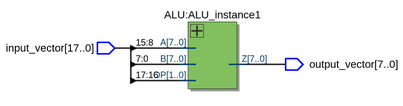
\includegraphics[width=0.6\linewidth]{alu.png}
        \caption{ALU}
        \label{fig:instru}
    \end{figure}
    \noindent
    As described earlier, ALU comprises of four operations which is then selected based on the multiplexer. The blocks present in ALU are listed below:
    \begin{itemize}
        \item 8-bit Adder
        \item Left Shifter
        \item Right Shifter
        \item 8-bit Multiplier
        \item 32-to-8 Multiplexer
    \end{itemize}
    \begin{figure}[H]
        \centering
        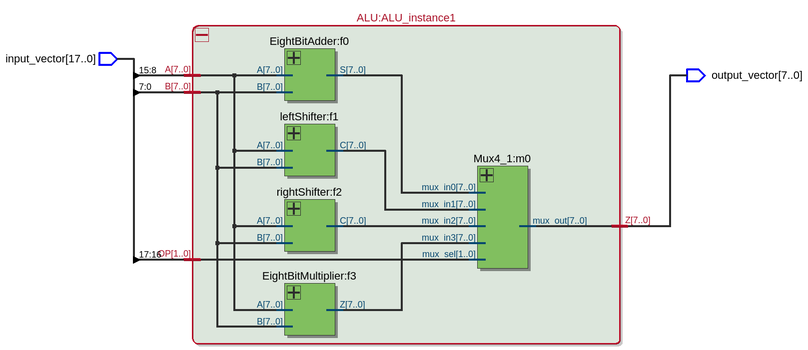
\includegraphics[width=0.6\linewidth]{alu_in.png}
        \caption{Blocks of ALU}
        \label{fig:instru}
    \end{figure}
        \newpage
        \noindent
        \textbf{Code of ALU}
        \noindent
        \begin{minted}{vhdl}
library ieee;
use ieee.std_logic_1164.all;

entity ALU is

	port(A, B : in std_logic_vector(7 downto 0);
		 OP : in std_logic_vector(1 downto 0);
		  Z : out std_logic_vector(7 downto 0));
		  
end entity ALU;

architecture struct of ALU is

	component Mux4_1
		port(
          mux_in0 : in std_logic_vector(7 downto 0);
          mux_in1 : in std_logic_vector(7 downto 0);
          mux_in2 : in std_logic_vector(7 downto 0);
          mux_in3 : in std_logic_vector(7 downto 0);
          mux_sel: in std_logic_vector(1 downto 0);
          mux_out : out std_logic_vector(7 downto 0) );

	end component;

	component EightBitAdder
		port(A, B : in std_logic_vector(7 downto 0);
		  S : out std_logic_vector(7 downto 0));
	end component;

	component leftShifter
		port(A, B : in std_logic_vector(7 downto 0);
		  C : out std_logic_vector(7 downto 0));
	end component;

	component rightShifter
		port(A, B : in std_logic_vector(7 downto 0);
		  C : out std_logic_vector(7 downto 0));
	end component;

	component EightBitMultiplier
		port(A, B : in std_logic_vector(7 downto 0);
		  Z : out std_logic_vector(7 downto 0));
	end component;

	signal inp0, inp1, inp2, inp3: std_logic_vector(7 downto 0);
	
begin

	f0 : EightBitAdder port map (A => A, B => B, S => inp0);
	f1 : leftShifter port map (A => A, B => B, C => inp1);
	f2 : rightShifter port map (A => A, B => B, C => inp2);
	f3 : EightBitMultiplier port map (A => A, B => B, Z => inp3);

	m0 : Mux4_1 port map (mux_in0 => inp0, mux_in1 => inp1, mux_in2 => inp2, mux_in3 => inp3, mux_sel => OP, mux_out => Z);
	
end struct;
        \end{minted}

%%%%%%%%%%%%%%%%%%%%%%%%%%%%%%%%%%%%%%%%%%%%%%%%%%%%%%%%%%%%%%%%%%%%%%%%%%%%%%%%%%%%%%%%%%%%%%%%%%
    \subsection{8-bit Adder}
        This component performs addition of two 8-bit inputs and returns the 8 LSB's of the sum.
        This is a ripple carry adder using eight full adders to perform 8-bit addition.\\\\
        \noindent
        \textbf{Block Diagram}
        \begin{figure}[H]
            \centering
            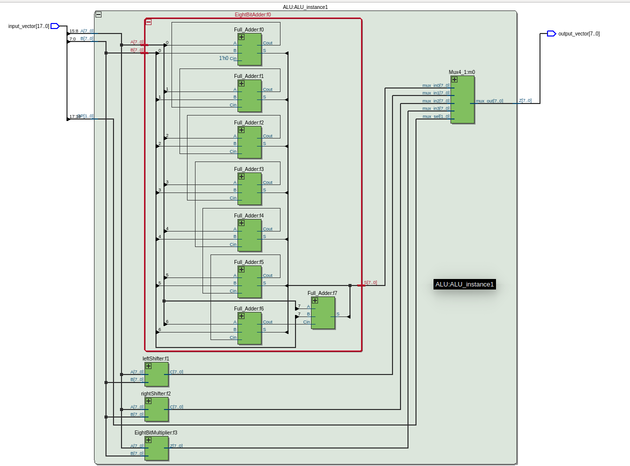
\includegraphics[width=0.6\linewidth]{eightbitadder.png}
            \caption{8-bit Adder}
            \label{fig:instru}
        \end{figure}
        \noindent
        \textbf{Code of Full Adder}
        \noindent
        \begin{minted}{vhdl}
library ieee;
use ieee.std_logic_1164.all;
library work;
use work.Gates.all;
entity Full_Adder  is
  port (A, B, Cin: in std_logic; S, Cout: out std_logic);
end entity Full_Adder;
architecture Struct of Full_Adder is
  signal tC, tS, U, V: std_logic;
begin

  ha: Half_Adder 
       port map (A => A, B => B, S => tS, C => tC);

  a1: welAnd2 port map (A => tS, B => Cin, Y => V);
  o1: welOr2  port map (A => V, B => tC, Y => Cout);
  
  x1: welXor2 port map (A => tS, B => Cin, Y => S);
end Struct;

        \end{minted}
    % \newpage
        \noindent
        \textbf{Code of 8-bit Adder}
        \noindent
\begin{minted}{vhdl}

library ieee;
use ieee.std_logic_1164.all;

entity EightBitAdder is

  port(A, B : in std_logic_vector(7 downto 0);
	      S : out std_logic_vector(7 downto 0));
		  
end entity EightBitAdder;

architecture struct of EightBitAdder is
  
  component Full_Adder
	port(A,B,Cin : in std_logic; Cout,S : out std_logic);
  end component;
	
  signal mid: std_logic_vector(6 downto 0);
	
begin

f0 : Full_Adder port map(A => A(0), B => B(0), Cin => '0', S => S(0), Cout => mid(0));
f1 : Full_Adder port map(A => A(1), B => B(1), Cin => mid(0), S => S(1), Cout => mid(1));
f2 : Full_Adder port map(A => A(2), B => B(2), Cin => mid(1), S => S(2), Cout => mid(2));
f3 : Full_Adder port map(A => A(3), B => B(3), Cin => mid(2), S => S(3), Cout => mid(3));
f4 : Full_Adder port map(A => A(4), B => B(4), Cin => mid(3), S => S(4), Cout => mid(4));
f5 : Full_Adder port map(A => A(5), B => B(5), Cin => mid(4), S => S(5), Cout => mid(5));
f6 : Full_Adder port map(A => A(6), B => B(6), Cin => mid(5), S => S(6), Cout => mid(6));
f7 : Full_Adder port map(A => A(7), B => B(7), Cin => mid(6), S => S(7), Cout => open);

end struct;
\end{minted}
        \noindent
        $\ast$ For Gates.vhdl, refer Appendix.
%%%%%%%%%%%%%%%%%%%%%%%%%%%%%%%%%%%%%%%%%%%%%%%%%%%%%%%%%%%%%%%%%%%%%%%%%%%%%%%%%%%%%%%%%%%%%%%%%%%%%%
    \subsection{Left Shifter}
        This component left shifts a 8-bit input by an amount specified by another 8-bit input and returns the 8 LSB's of the shifted number.\\\\
        This is implemented by a combination of three type of shifters : Shift Left by 1 bit, Shift Left by 2 bits and Shift Left by 4 bits.\\\\
        \noindent
        \textbf{Block Diagram}
        \begin{figure}[H]
            \centering
            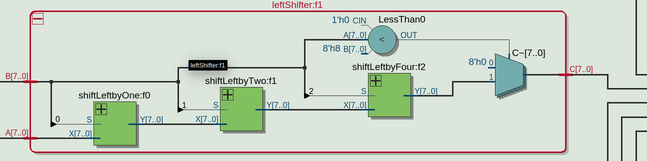
\includegraphics[width=0.6\linewidth]{leftshifter.png}
            \caption{Left Shifter}
            \label{fig:instru}
        \end{figure}
        % \begin{figure}[H]
        %     \centering
        %     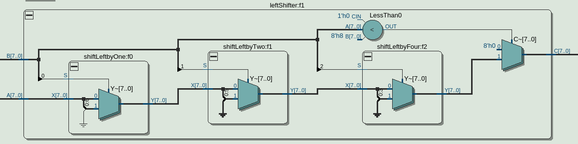
\includegraphics[width=0.6\linewidth]{leftShifterFull.png}
        %     \caption{Inside of Left Shifter}
        %     \label{fig:instru}
        % \end{figure}
        
        \noindent
        \textbf{Code of Shift Left by 1}
        \noindent
        \begin{minted}{vhdl}
library ieee;
use ieee.std_logic_1164.all;

entity shiftLeftbyOne is

	port(X : in std_logic_vector(7 downto 0);
		 S : in std_logic;
		  Y : out std_logic_vector(7 downto 0));
		  
end entity shiftLeftbyOne;

architecture easy of shiftLeftbyOne is

begin
	Y(7) <= X(6) when S='1' else X(7);
	Y(6) <= X(5) when S='1' else X(6);
	Y(5) <= X(4) when S='1' else X(5);
	Y(4) <= X(3) when S='1' else X(4);
	Y(3) <= X(2) when S='1' else X(3);
	Y(2) <= X(1) when S='1' else X(2);
	Y(1) <= X(0) when S='1' else X(1);
	Y(0) <= '0' when S='1' else X(0);
end easy;
        \end{minted}
        
        \noindent
        \textbf{Code of Shift Left by 2}
        \noindent
        \begin{minted}{vhdl}
library ieee;
use ieee.std_logic_1164.all;

entity shiftLeftbyTwo is

	port(X : in std_logic_vector(7 downto 0);
		 S : in std_logic;
		  Y : out std_logic_vector(7 downto 0));
		  
end entity shiftLeftbyTwo;

architecture easy of shiftLeftbyTwo is

begin
	Y(7) <= X(5) when S='1' else X(7);
	Y(6) <= X(4) when S='1' else X(6);
	Y(5) <= X(3) when S='1' else X(5);
	Y(4) <= X(2) when S='1' else X(4);
	Y(3) <= X(1) when S='1' else X(3);
	Y(2) <= X(0) when S='1' else X(2);
	Y(1) <= '0' when S='1' else X(1);
	Y(0) <= '0' when S='1' else X(0);
end easy;
        \end{minted}
        
        \noindent
        \textbf{Code of Shift Left by 4}
        \noindent
        \begin{minted}{vhdl}
library ieee;
use ieee.std_logic_1164.all;

entity shiftLeftbyFour is

	port(X : in std_logic_vector(7 downto 0);
		 S : in std_logic;
		  Y : out std_logic_vector(7 downto 0));
		  
end entity shiftLeftbyFour;

architecture easy of shiftLeftbyFour is

begin
	Y(7) <= X(3) when S='1' else X(7);
	Y(6) <= X(2) when S='1' else X(6);
	Y(5) <= X(1) when S='1' else X(5);
	Y(4) <= X(0) when S='1' else X(4);
	Y(3) <= '0' when S='1' else X(3);
	Y(2) <= '0' when S='1' else X(2);
	Y(1) <= '0' when S='1' else X(1);
	Y(0) <= '0' when S='1' else X(0);
end easy;
        \end{minted}

    % \newpage
        \noindent
        \textbf{Code of Complete Left Shifter}
        \noindent
        \begin{minted}{vhdl}

library ieee;
use ieee.std_logic_1164.all;

entity leftShifter is

	port(A, B : in std_logic_vector(7 downto 0);
		  C : out std_logic_vector(7 downto 0));
		  
end entity leftShifter;

architecture easy of leftShifter is
	component shiftLeftbyOne
		port(X : in std_logic_vector(7 downto 0);
		 	S : in std_logic;
		  	Y : out std_logic_vector(7 downto 0));
	end component;

	component shiftLeftbyTwo
		port(X : in std_logic_vector(7 downto 0);
		 	S : in std_logic;
		  	Y : out std_logic_vector(7 downto 0));
	end component;

	component shiftLeftbyFour
		port(X : in std_logic_vector(7 downto 0);
		 	S : in std_logic;
		  	Y : out std_logic_vector(7 downto 0));
	end component;

	signal mid0: std_logic_vector(7 downto 0);
	signal mid1: std_logic_vector(7 downto 0);
	signal mid2: std_logic_vector(7 downto 0);

begin

	f0 : shiftLeftbyOne port map(X => A, S => B(0), Y => mid0);
	f1 : shiftLeftbyTwo port map(X => mid0, S => B(1), Y => mid1);
	f2 : shiftLeftbyFour port map(X => mid1, S => B(2), Y => mid2);

	C <= mid2 when (B < "00001000") else "00000000";

end easy;
        \end{minted}

%%%%%%%%%%%%%%%%%%%%%%%%%%%%%%%%%%%%%%%%%%%%%%%%%%%%%%%%%%%%%%%%%%%%%%%%%%%%%%%%%%%%%%%%%%%%%%%%%%%%%
    \newpage
    \subsection{Right Shifter}
        This component right shifts a 8-bit input by an amount specified by another 8-bit input and returns the 8 LSB's of the shifted number.\\\\
        This is implemented by a combination of three type of shifters : Shift Right by 1 bit, Shift Right by 2 bits and Shift Right by 4 bits.\\\\
        \noindent
        \textbf{Block Diagram}
        \begin{figure}[H]
            \centering
            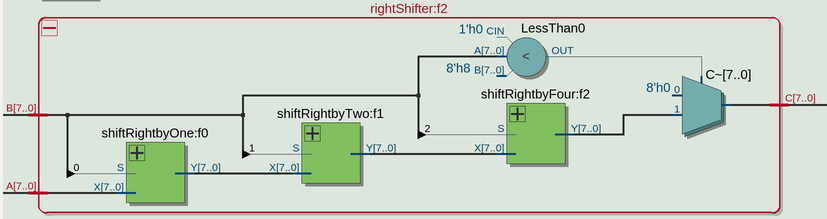
\includegraphics[width=0.6\linewidth]{rightShifter.png}
            \caption{Right Shifter}
            \label{fig:instru}
        \end{figure}
        % \begin{figure}[H]
        %     \centering
        %     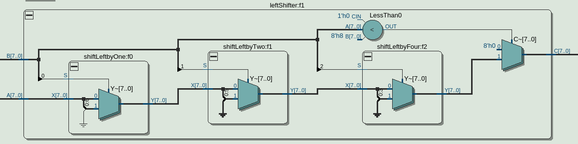
\includegraphics[width=0.6\linewidth]{leftShifterFull.png}
        %     \caption{Inside of Left Shifter}
        %     \label{fig:instru}
        % \end{figure}
        
        \noindent
        \textbf{Code of Shift Right by 1}
        \noindent
        \begin{minted}{vhdl}
library ieee;
use ieee.std_logic_1164.all;

entity shiftRightbyOne is

	port(X : in std_logic_vector(7 downto 0);
		 S : in std_logic;
		  Y : out std_logic_vector(7 downto 0));
		  
end entity shiftRightbyOne;

architecture easy of shiftRightbyOne is

begin
	Y(7) <= '0' when S='1' else X(7);
	Y(6) <= X(7) when S='1' else X(6);
	Y(5) <= X(6) when S='1' else X(5);
	Y(4) <= X(5) when S='1' else X(4);
	Y(3) <= X(4) when S='1' else X(3);
	Y(2) <= X(3) when S='1' else X(2);
	Y(1) <= X(2) when S='1' else X(1);
	Y(0) <= X(1) when S='1' else X(0);
end easy;
        \end{minted}
        
        \noindent
        \textbf{Code of Shift Right by 2}
        \noindent
        \begin{minted}{vhdl}
library ieee;
use ieee.std_logic_1164.all;

entity shiftRightbyTwo is

	port(X : in std_logic_vector(7 downto 0);
		 S : in std_logic;
		  Y : out std_logic_vector(7 downto 0));
		  
end entity shiftRightbyTwo;

architecture easy of shiftRightbyTwo is

begin
	Y(7) <= '0' when S='1' else X(7);
	Y(6) <= '0' when S='1' else X(6);
	Y(5) <= X(7) when S='1' else X(5);
	Y(4) <= X(6) when S='1' else X(4);
	Y(3) <= X(5) when S='1' else X(3);
	Y(2) <= X(4) when S='1' else X(2);
	Y(1) <= X(3) when S='1' else X(1);
	Y(0) <= X(2) when S='1' else X(0);
end easy;
        \end{minted}
        
        \noindent
        \textbf{Code of Shift Right by 4}
        \noindent
        \begin{minted}{vhdl}
library ieee;
use ieee.std_logic_1164.all;

entity shiftRightbyFour is

	port(X : in std_logic_vector(7 downto 0);
		 S : in std_logic;
		  Y : out std_logic_vector(7 downto 0));
		  
end entity shiftRightbyFour;

architecture easy of shiftRightbyFour is

begin
	Y(7) <= '0' when S='1' else X(7);
	Y(6) <= '0' when S='1' else X(6);
	Y(5) <= '0' when S='1' else X(5);
	Y(4) <= '0' when S='1' else X(4);
	Y(3) <= X(7) when S='1' else X(3);
	Y(2) <= X(6) when S='1' else X(2);
	Y(1) <= X(5) when S='1' else X(1);
	Y(0) <= X(4) when S='1' else X(0);
end easy;
        \end{minted}

    % \newpage
        \noindent
        \textbf{Code of Complete Right Shifter}
        \noindent
        \begin{minted}{vhdl}
library ieee;
use ieee.std_logic_1164.all;

entity rightShifter is

	port(A, B : in std_logic_vector(7 downto 0);
		  C : out std_logic_vector(7 downto 0));
		  
end entity rightShifter;

architecture easy of RightShifter is
	component shiftRightbyOne
		port(X : in std_logic_vector(7 downto 0);
		 	S : in std_logic;
		  	Y : out std_logic_vector(7 downto 0));
	end component;

	component shiftRightbyTwo
		port(X : in std_logic_vector(7 downto 0);
		 	S : in std_logic;
		  	Y : out std_logic_vector(7 downto 0));
	end component;

	component shiftRightbyFour
		port(X : in std_logic_vector(7 downto 0);
		 	S : in std_logic;
		  	Y : out std_logic_vector(7 downto 0));
	end component;

	signal mid0: std_logic_vector(7 downto 0);
	signal mid1: std_logic_vector(7 downto 0);
	signal mid2: std_logic_vector(7 downto 0);

begin

	f0 : shiftRightbyOne port map(X => A, S => B(0), Y => mid0);
	f1 : shiftRightbyTwo port map(X => mid0, S => B(1), Y => mid1);
	f2 : shiftRightbyFour port map(X => mid1, S => B(2), Y => mid2);

	C <= mid2 when (B < "00001000") else "00000000";

end easy;
        \end{minted}

%%%%%%%%%%%%%%%%%%%%%%%%%%%%%%%%%%%%%%%%%%%%%%%%%%%%%%%%%%%%%%%%%%%%%%%%%%%%%%%%%%%%%%%%%%%%%%%%%%%%%%%%   
    \subsection{8-bit Multiplier}
        This component performs multiplication of two 8-bit inputs and returns the 8 LSB's of the product.\\\\
        This is implemented using left shifter, and two additional components which are described below:
        \begin{itemize}
            \item When we perform multiplication of bits, we multiply the first number by first bit, and then by second bit and shift left this product by 1 and so on.
            \item So, checkBool is designed to return the same number if the multiplying bit is '1' or else return 0 (8-bits)
            \item We the use left shifter to shift products resulting from multiplication by each bit.
            \item At last we add these 8 numbers of 8-bit each using a 8-input adder.
        \end{itemize}
        \noindent
        \textbf{Block Diagram}
        \begin{figure}[H]
            \centering
            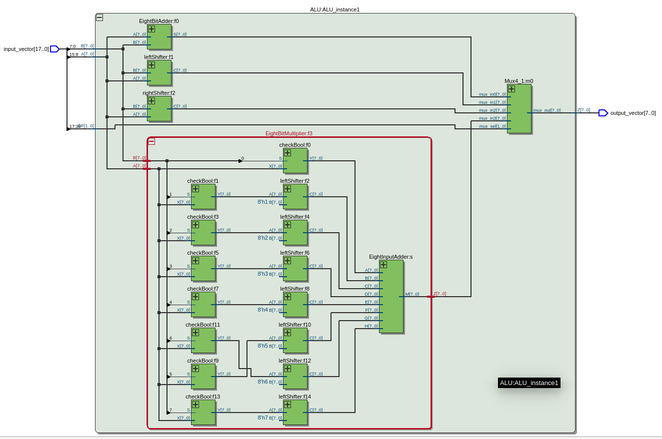
\includegraphics[width=0.8\linewidth, height=5in]{eightmultiplier.png}
            \caption{8-bit Multiplier}
            \label{fig:instru}
        \end{figure} 
    
        \noindent
        \textbf{Code of checkBool}
        \noindent
        \begin{minted}{vhdl}
library ieee;
use ieee.std_logic_1164.all;

entity checkBool is

	port(X : in std_logic_vector(7 downto 0);
		 S : in std_logic;
		  Y : out std_logic_vector(7 downto 0));
		  
end entity checkBool;

architecture easy of checkBool is

begin

	Y <= X when S='1' else "00000000";

end easy;
        \end{minted}

        \noindent
        \textbf{Code of 8-input 8-bit adder}
        \noindent
        \begin{minted}{vhdl}
library ieee;
use ieee.std_logic_1164.all;

entity EightInputAdder is

	port(A, B, C, D, E, F, G, H : in std_logic_vector(7 downto 0);
		  M : out std_logic_vector(7 downto 0));
		  
end entity EightInputAdder;

architecture struct of EightInputAdder is

	component EightBitAdder
		port(A, B : in std_logic_vector(7 downto 0);
		  S : out std_logic_vector(7 downto 0));
	end component;
	
	signal sum0, sum1, sum2, sum3, sum4, sum5, sum6: std_logic_vector(7 downto 0);
	
begin

	f0 : EightBitAdder port map (A => A, B => B, S => sum0);
	f1 : EightBitAdder port map (A => sum0, B => C, S => sum1);
	f2 : EightBitAdder port map (A => sum1, B => D, S => sum2);
	f3 : EightBitAdder port map (A => sum2, B => E, S => sum3);
	f4 : EightBitAdder port map (A => sum3, B => F, S => sum4);
	f5 : EightBitAdder port map (A => sum4, B => G, S => sum5);
	f6 : EightBitAdder port map (A => sum5, B => H, S => M);
	
end struct;      
        \end{minted}
        % \newpage
        \noindent
        \textbf{Block Diagram}
        \begin{figure}[H]
            \centering
            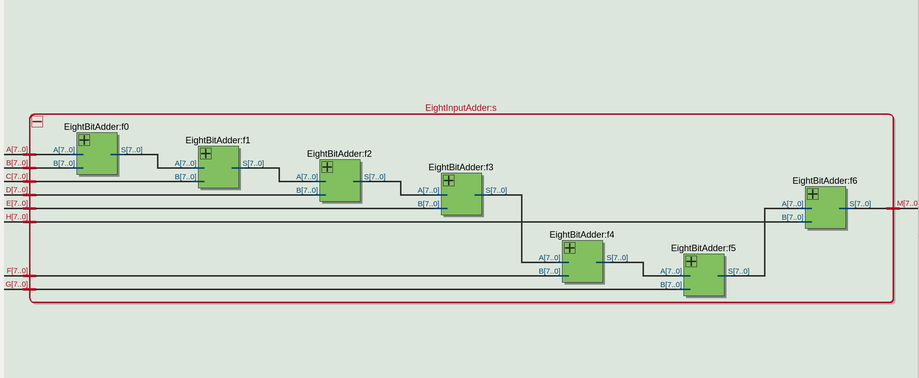
\includegraphics[width=0.8\linewidth]{eightInputAdder.png}
            \caption{8-bit Multiplier}
            \label{fig:instru}
        \end{figure} 
        % \newpage
        \noindent
        \textbf{Code of 8-bit Multiplier}
        \noindent
        \begin{minted}{vhdl}
library ieee;
use ieee.std_logic_1164.all;

entity EightBitMultiplier is

	port(A, B : in std_logic_vector(7 downto 0);
		  Z : out std_logic_vector(7 downto 0));
		  
end entity EightBitMultiplier;

architecture struct of EightBitMultiplier is

	component EightInputAdder
		port(A, B, C, D, E, F, G, H : in std_logic_vector(7 downto 0);
		  M : out std_logic_vector(7 downto 0));
	end component;

	component leftShifter
		port(A, B : in std_logic_vector(7 downto 0);
		  C : out std_logic_vector(7 downto 0));
	end component;

	component checkBool
		port(X : in std_logic_vector(7 downto 0);
		 S : in std_logic;
		  Y : out std_logic_vector(7 downto 0));
	end component;

	signal mid0, mid1, mid2, mid3, mid4, mid5, mid6: std_logic_vector(7 downto 0);
	signal sum0, sum1, sum2, sum3: std_logic_vector(7 downto 0);
	signal sum4, sum5, sum6, sum7: std_logic_vector(7 downto 0);
	
begin

	f0 : checkBool port map (X => A, S => B(0), Y => sum0);
	f1 : checkBool port map (X => A, S => B(1), Y => mid0);
	f2 : leftShifter port map (A => mid0, B => "00000001", C => sum1); 
	f3 : checkBool port map (X => A, S => B(2), Y => mid1);
	f4 : leftShifter port map (A => mid1, B => "00000010", C => sum2); 
	f5 : checkBool port map (X => A, S => B(3), Y => mid2);
	f6 : leftShifter port map (A => mid2, B => "00000011", C => sum3); 
	f7 : checkBool port map (X => A, S => B(4), Y => mid3);
	f8 : leftShifter port map (A => mid3, B => "00000100", C => sum4); 
	f9 : checkBool port map (X => A, S => B(5), Y => mid4);
	f10 : leftShifter port map (A => mid4, B => "00000101", C => sum5); 
	f11 : checkBool port map (X => A, S => B(6), Y => mid5);
	f12 : leftShifter port map (A => mid5, B => "00000110", C => sum6); 
	f13 : checkBool port map (X => A, S => B(7), Y => mid6);
	f14 : leftShifter port map (A => mid6, B => "00000111", C => sum7);

	s : EightInputAdder port map (A => sum0, B => sum1, C => sum2, D => sum3,
	E => sum4, F => sum5, G => sum6, H => sum7, M => Z); 
	
end struct;
        \end{minted}
    
%%%%%%%%%%%%%%%%%%%%%%%%%%%%%%%%%%%%%%%%%%%%%%%%%%%%%%%%%%%%%%%%%%%%%%%%%%%%%%%%%%%%%%%%%%%%%%%%%%%%%%
    \newpage
    \subsection{32-to-8 Multiplexer}
        This component decides according to the opcode (select lines) as to which operation is to be performed.\\\\
        It takes 34 inputs i.e. four 8-bit inputs corresponding to four operations and two opcode bits for selecting which operation to perform and returns a 8-bit number corresponding to the operation selected.\\\\
        \noindent
        \textbf{Block Diagram}
        \begin{figure}[H]
            \centering
            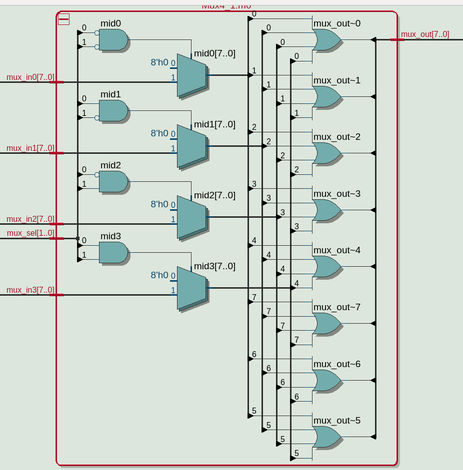
\includegraphics[width=0.8\linewidth, height=6in]{mux.png}
            \caption{32-to-8 Multiplexer}
            \label{fig:instru}
        \end{figure} 
        \newpage
        \noindent
        \textbf{Code of MUX}
        \noindent
        \begin{minted}{vhdl}
library ieee;
use ieee.std_logic_1164.all;library ieee;
use ieee.std_logic_1164.all;

entity Mux4_1 is
	
	port(
          mux_in0 : in std_logic_vector(7 downto 0);
          mux_in1 : in std_logic_vector(7 downto 0);
          mux_in2 : in std_logic_vector(7 downto 0);
          mux_in3 : in std_logic_vector(7 downto 0);
          mux_sel: in std_logic_vector(1 downto 0);
          mux_out : out std_logic_vector(7 downto 0) );

end entity Mux4_1;	

architecture dataflow of Mux4_1 is

	signal mid0: std_logic_vector(7 downto 0);
	signal mid1: std_logic_vector(7 downto 0);
	signal mid2: std_logic_vector(7 downto 0);
	signal mid3: std_logic_vector(7 downto 0);

begin 

	mid0 <= mux_in0 when (not mux_sel(0) and not mux_sel(1)) = '1' else "00000000";
	mid1 <= mux_in1 when (mux_sel(0) and not mux_sel(1)) = '1' else "00000000";
	mid2 <= mux_in2 when (not mux_sel(0) and mux_sel(1)) = '1' else "00000000";
	mid3 <= mux_in3 when (mux_sel(0) and mux_sel(1)) = '1' else "00000000";
	
	mux_out <= mid0 or mid1 or mid2 or mid3;
	
end architecture dataflow;
        \end{minted}

%%%%%%%%%%%%%%%%%%%%%%%%%%%%%%%%%%%%%%%%%%%%%%%%%%%%%%%%%%%%%%%%%%%%%%%%%%%%%%%%%%%%%%%%%%%%%%%%%%%%%%%%%   
\newpage
\section{Simulation}
    For simulation we define a DUT instance and create a testbench file to test our design taking inputs from tracefile and verifying it.\\\\
    \noindent
    \textbf{Code of DUT}
    \noindent
    \begin{minted}{vhdl}
library ieee;
use ieee.std_logic_1164.all;
entity DUT is
   port(input_vector: in std_logic_vector(17 downto 0);
           output_vector: out std_logic_vector ( 7 downto 0) );
end entity;

architecture DutWrap of DUT is
   component ALU is
          port(A, B : in std_logic_vector(7 downto 0);
            OP : in std_logic_vector(1 downto 0);
            Z : out std_logic_vector(7 downto 0));
   end component;
begin
   ALU_instance1 : ALU
             port map (
                OP   => input_vector(17 downto 16),
                A   => input_vector(15 downto 8),
                B   => input_vector(7 downto 0),
                Z => output_vector(7 downto 0) );
end DutWrap;
    \end{minted}
    \noindent
    \textbf{Code of Testbench}
    \noindent
    \begin{minted}{vhdl}
library std;
use std.textio.all;

library ieee;
use ieee.std_logic_1164.all;

entity Testbench is
end entity;
architecture Behave of Testbench is

  ----------------------------------------------------------------
  --  edit the following lines to set the number of i/o's of your
  --  DUT.
  ----------------------------------------------------------------
  constant number_of_inputs  : integer := 18;  -- # input bits to your design.
  constant number_of_outputs : integer := 8;  -- # output bits from your design.
  ----------------------------------------------------------------
  ----------------------------------------------------------------

  -- Note that you will have to wrap your design into the DUT
  -- as indicated in class.
  component DUT is
   port(input_vector: in std_logic_vector(number_of_inputs-1 downto 0);    
       	output_vector: out std_logic_vector(number_of_outputs-1 downto 0));
  end component;


  signal input_vector  : std_logic_vector(number_of_inputs-1 downto 0);
  signal output_vector : std_logic_vector(number_of_outputs-1 downto 0);

  -- create a constrained string
  function to_string(x: string) return string is
      variable ret_val: string(1 to x'length);
      alias lx : string (1 to x'length) is x;
  begin  
      ret_val := lx;
      return(ret_val);
  end to_string;

  -- bit-vector to std-logic-vector and vice-versa
  function to_std_logic_vector(x: bit_vector) return std_logic_vector is
     alias lx: bit_vector(1 to x'length) is x;
     variable ret_val: std_logic_vector(1 to x'length);
  begin
     for I in 1 to x'length loop
        if(lx(I) = '1') then
          ret_val(I) := '1';
        else
          ret_val(I) := '0';
        end if;
     end loop; 
     return ret_val;
  end to_std_logic_vector;

  function to_bit_vector(x: std_logic_vector) return bit_vector is
     alias lx: std_logic_vector(1 to x'length) is x;
     variable ret_val: bit_vector(1 to x'length);
  begin
     for I in 1 to x'length loop
        if(lx(I) = '1') then
          ret_val(I) := '1';
        else
          ret_val(I) := '0';
        end if;
     end loop; 
     return ret_val;
  end to_bit_vector;

begin
  process 
    variable err_flag : boolean := false;
    File INFILE: text open read_mode is "TRACEFILE.txt";
    FILE OUTFILE: text  open write_mode is "OUTPUTS.txt";

    -- bit-vectors are read from the file.
    variable input_vector_var: bit_vector (number_of_inputs-1 downto 0);
    variable output_vector_var: bit_vector (number_of_outputs-1 downto 0);
    variable output_mask_var: bit_vector (number_of_outputs-1 downto 0);

    -- for comparison of output with expected-output
    variable output_comp_var: std_logic_vector (number_of_outputs-1 downto 0);
    constant ZZZZ : std_logic_vector(number_of_outputs-1 downto 0) := (others => '0');

    -- for read/write.
    variable INPUT_LINE: Line;
    variable OUTPUT_LINE: Line;
    variable LINE_COUNT: integer := 0;

    
  begin
    while not endfile(INFILE) loop 
	  -- will read a new line every 5ns, apply input,
	  -- wait for 1 ns for circuit to settle.
	  -- read output.


          LINE_COUNT := LINE_COUNT + 1;


	  -- read input at current time.
	  readLine (INFILE, INPUT_LINE);
          read (INPUT_LINE, input_vector_var);
          read (INPUT_LINE, output_vector_var);
          read (INPUT_LINE, output_mask_var);
	
	  -- apply input.
          input_vector <= to_std_logic_vector(input_vector_var);

	  -- wait for the circuit to settle 
	  wait for 40 ns;

	  -- check output.
          output_comp_var := (to_std_logic_vector(output_mask_var) and 
		    (output_vector xor to_std_logic_vector(output_vector_var)));
	  if (output_comp_var  /= ZZZZ) then
             write(OUTPUT_LINE,to_string("ERROR: line "));
             write(OUTPUT_LINE, LINE_COUNT);
             writeline(OUTFILE, OUTPUT_LINE);
             err_flag := true;
          end if;

          write(OUTPUT_LINE, to_bit_vector(input_vector));
          write(OUTPUT_LINE, to_string(" "));
          write(OUTPUT_LINE, to_bit_vector(output_vector));
          writeline(OUTFILE, OUTPUT_LINE);

	  -- advance time by 4 ns.
	  wait for 4 ns;
    end loop;

    assert (err_flag) report "SUCCESS, all tests passed." severity note;
    assert (not err_flag) report "FAILURE, some tests failed." severity error;

    wait;
  end process;

  dut_instance: DUT 
     	port map(input_vector => input_vector, 
     	         output_vector => output_vector);

end Behave;

    \end{minted}
    \noindent
    $\ast$ For Tracefile, refer Appendix.
    
    \newpage 
    \subsection{RTL Simulation}
    \noindent
    \begin{figure}[H]
        \centering
        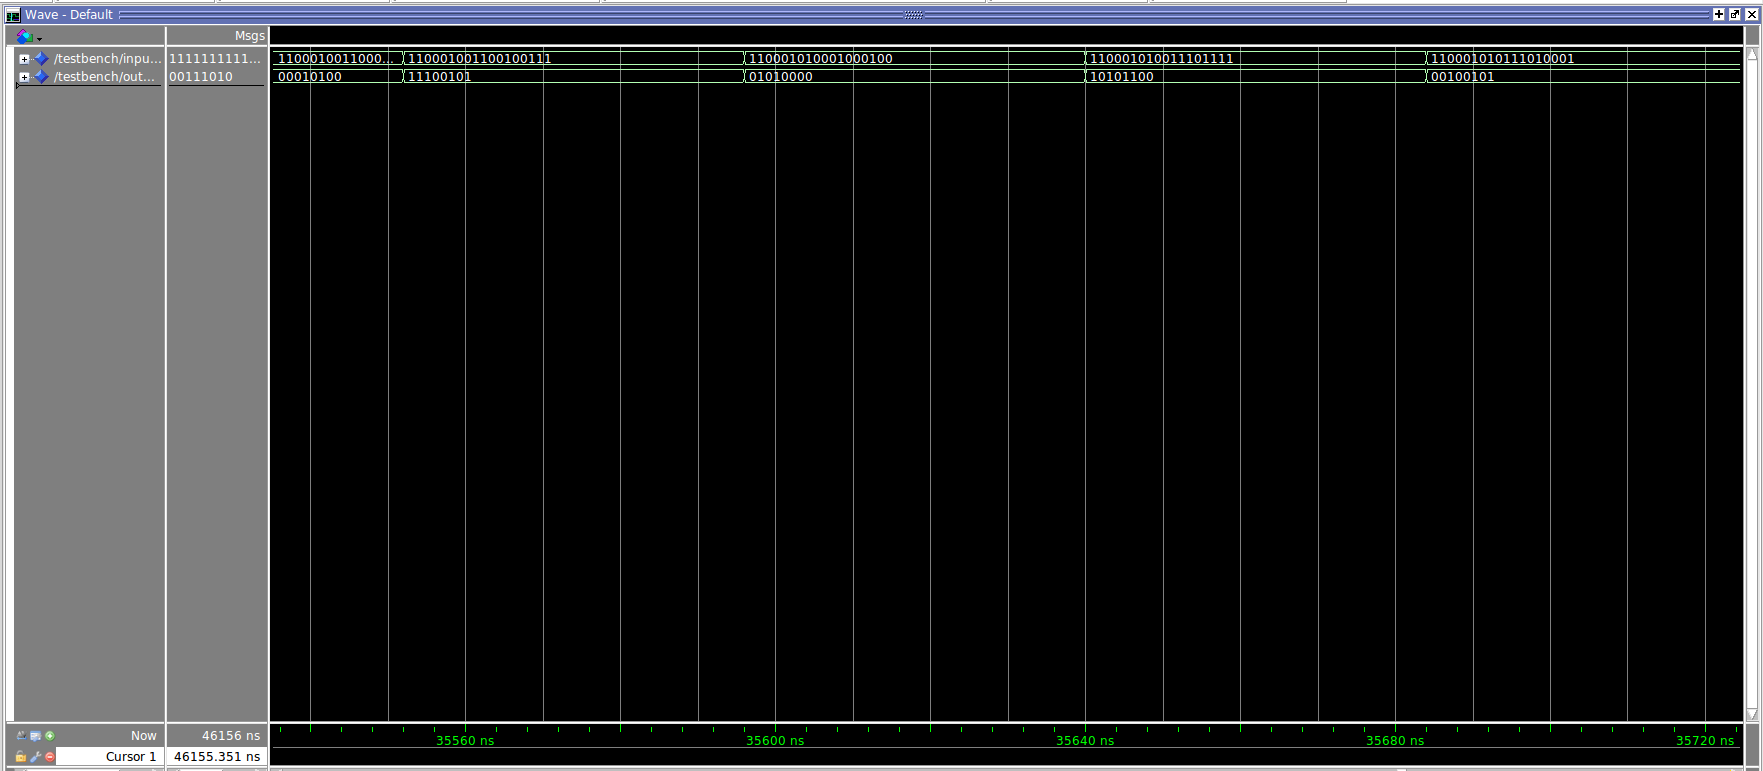
\includegraphics[width=0.8\linewidth]{rtl_simproper.png}
    \end{figure}
    % \begin{figure}[H]
    %     \centering
    %     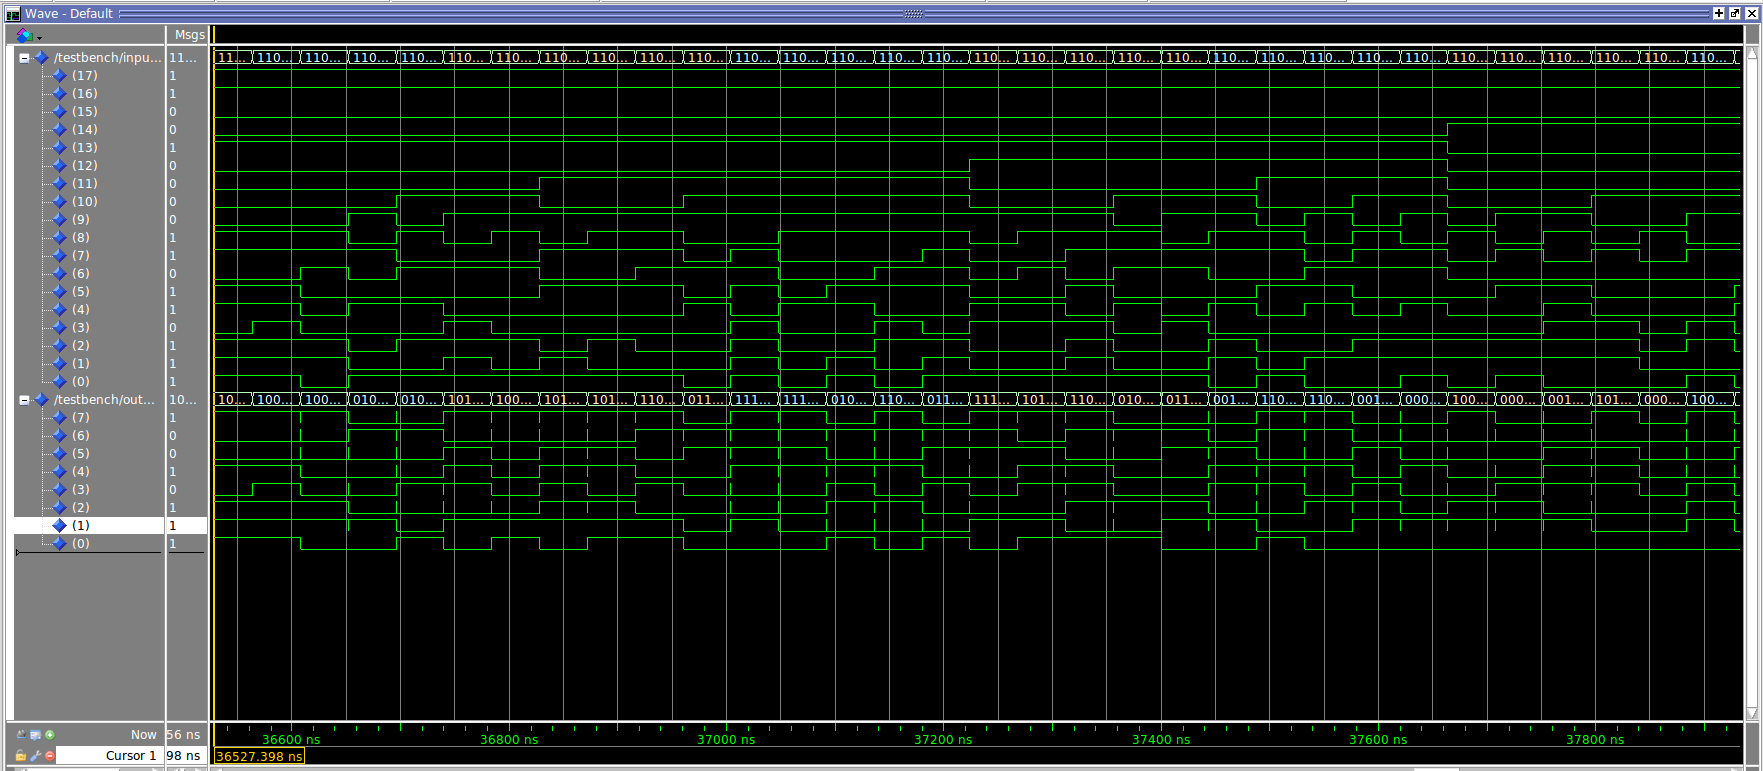
\includegraphics[width=0.8\linewidth]{rlt_sim.png}
    % \end{figure}
    
    \begin{figure}[H]
        \centering
        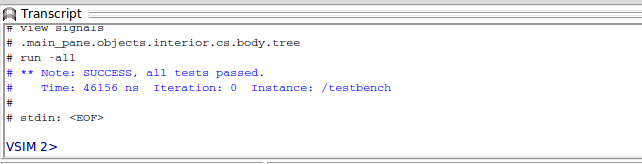
\includegraphics[width=0.8\linewidth]{rtl_simproper (copy).png}
    \end{figure}
    \subsection{Gate Level Simulation}
    \noindent
    \begin{figure}[H]
        \centering
        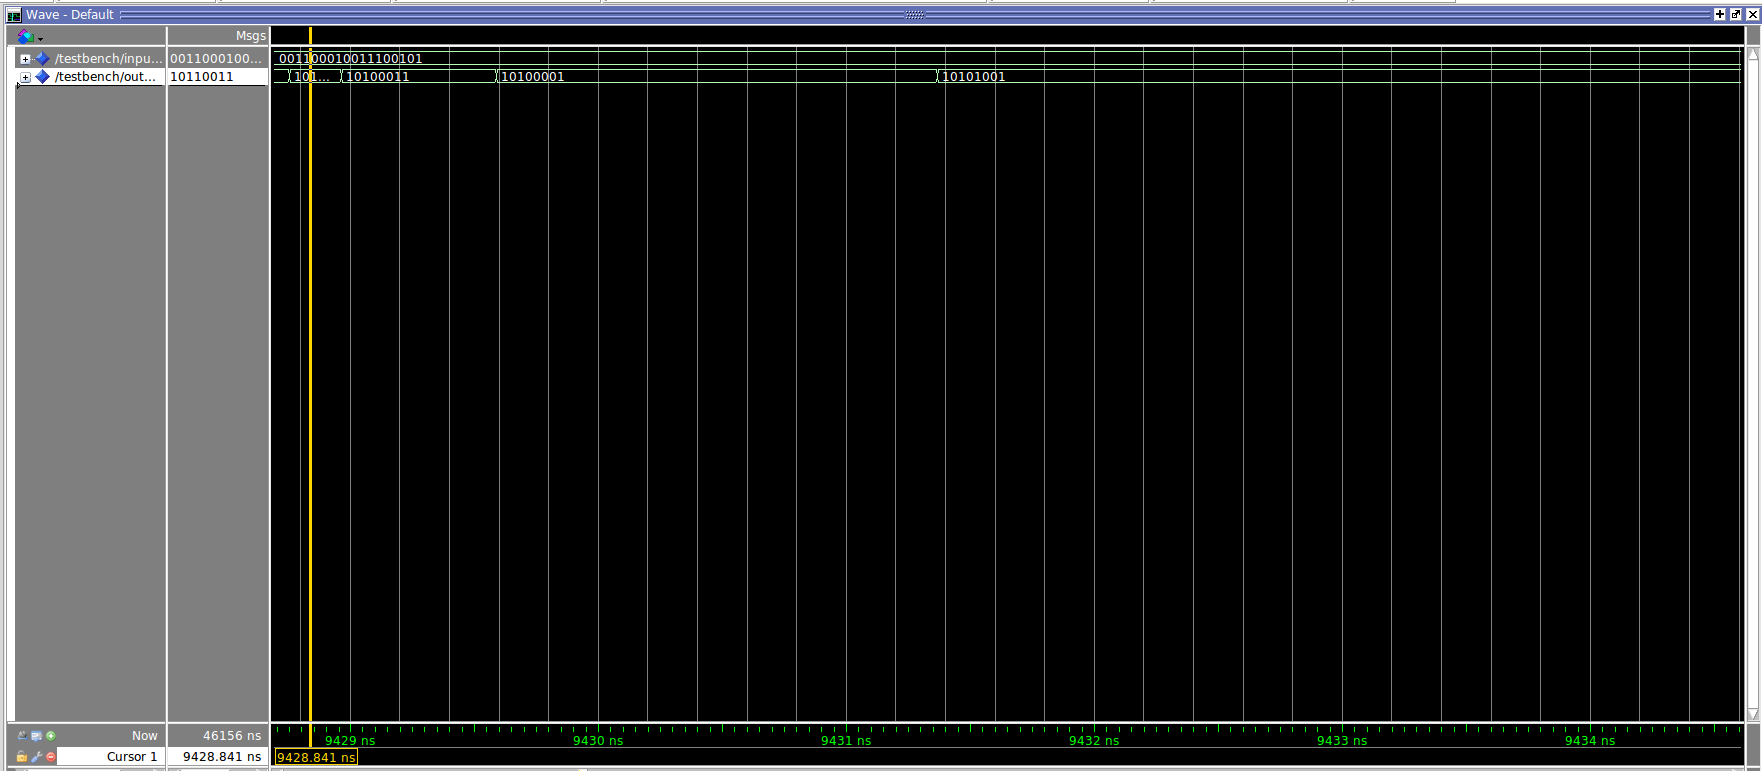
\includegraphics[width=0.8\linewidth]{gateLevel.png}
    \end{figure}
    % \begin{figure}[H]
    %     \centering
    %     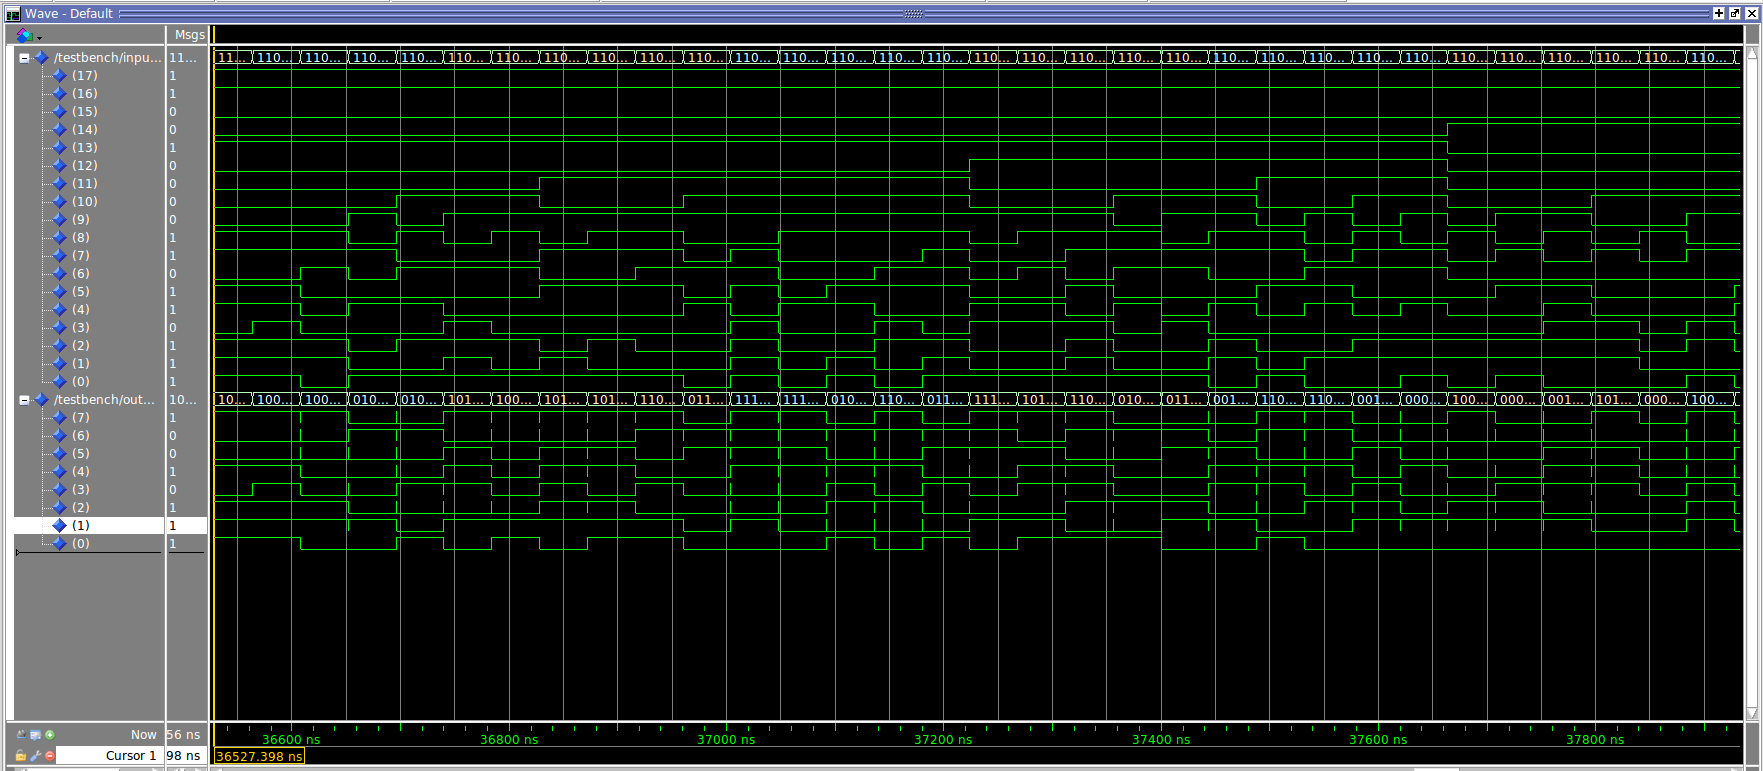
\includegraphics[width=0.8\linewidth]{rlt_sim.png}
    % \end{figure}
    
    \begin{figure}[H]
        \centering
        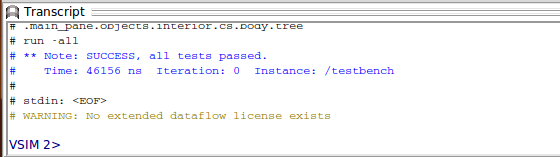
\includegraphics[width=0.8\linewidth]{gateLevel (copy).png}
    \end{figure}
    
%%%%%%%%%%%%%%%%%%%%%%%%%%%%%%%%%%%%%%%%%%%%%%%%%%%%%%%%%%%%%%%%%%%%%%%%%%%%%%%%%%%%%%%%%%%%%%%%%%%%%%%%
\newpage
\section{Verification}
    Here to verify our design we test it on Krypton Board using scan chain files which are given below
    \subsection{Scan Chain}
        \noindent
        \textbf{Code of Scan Reg}
        \noindent
        \begin{minted}{vhdl}
----------------------------------------
-- Scan Chain Module : WEL Lab
-- Author : Raunak Gupta, Soumik Sarkar
-- Date : 20/3/2016
----------------------------------------
library ieee;
use ieee.std_logic_1164.all;
use ieee.numeric_std.all;

entity Scan_Reg is
  generic (length	: integer);             -- length of the register
  port (
    clock, reset	: in std_ulogic;						
    -- clock and reset input
    PI			: in  unsigned(length-1 downto 0);  		
    -- parallel data input
    PO			: out  unsigned(length-1 downto 0);		
    -- parallel data output
    SI			: in std_ulogic ;					
    -- serial data input
    SO			: out std_ulogic;					
    -- serial data output
    L1_en, L2_en	: in std_ulogic;						
    -- Enable signal for two flip-flops
    cap_shft		: in std_ulogic;						
    -- Capture / Shift signal
    sel_reg		: in std_ulogic						
    -- Select register
    );
end Scan_Reg;

architecture behave of Scan_Reg is

signal mux1, mux2, L1, L2 : unsigned(length-1 downto 0); 
begin	--behave

	Multiplexor_1 : process (PI, SI, cap_shft, L1)
	begin
		if (cap_shft = '0') then
			mux1 <= PI;
		else
			mux1 <= SI & L1(length-1 downto 1);
		end if;
	end process Multiplexor_1;

	Latch_1 : process (clock, reset)
	begin
		if (clock'event and clock = '1') then
			if (reset = '1') then
				L1 <= unsigned(to_unsigned(0, length));
			elsif (L1_en  = '1' ) then
				L1 <= mux1;
			else
				L1 <= L1;
			end if;
		end if;
	end process Latch_1;

	Latch_2 : process (clock, reset)
	begin
		if (clock'event and clock = '1') then
			if (reset = '1') then
				L2 <= unsigned(to_unsigned(0, length));
			elsif (L2_en  = '1' ) then
				L2 <= L1;
			else
				L2 <= L2;
			end if;
		end if;
	end process Latch_2;

	Multiplexor_2 : process (L2, PI, sel_reg)
	begin
		if (sel_reg = '0') then
			mux2 <= PI;
		else
			mux2 <= L2;
		end if;
	end process Multiplexor_2;

	PO <= mux2;
	SO <= L1(0);

end architecture behave;
        \end{minted}

        \noindent
        \textbf{Code of Scan Chain}
        \noindent
        \begin{minted}{vhdl}
----------------------------------------
-- Scan Chain Module : WEL Lab
-- Author : Raunak Gupta, Soumik Sarkar
-- Date : 20/3/2016
----------------------------------------
library ieee;
use ieee.std_logic_1164.all;
use ieee.numeric_std.all;

entity Scan_Chain is
  generic (
    in_pins	: integer;			-- Number of input pins
    out_pins	: integer			-- Number of output pins
 );
  port (
    TDI		: in std_ulogic;		-- Test Data In
    TDO		: out std_ulogic;		-- Test Data Out
    TMS		: in std_ulogic;		-- TAP controller signal
    TCLK		: in std_ulogic;		   -- Test clock
    TRST		: in std_ulogic;	    -- Test reset
    dut_in	: out unsigned(in_pins-1 downto 0);	-- Input for the DUT
    dut_out	: in unsigned(out_pins-1 downto 0)	-- Output from the DUT
    );
end Scan_Chain;

architecture behave of Scan_Chain is

component Scan_reg is												
    -- register as a component
  generic (
    length	: integer												
    -- length of the register
    );
  port (
    clock, reset	: in std_ulogic;								
    -- clock and reset input
    PI				: in  unsigned(length-1 downto 0);  	
    -- parallel data input
    PO				: out  unsigned(length-1 downto 0);		
    -- parallel data output
    SI				: in std_ulogic ;								
    -- serial data input
    SO				: out std_ulogic;								
    -- serial data output
    L1_en, L2_en	: in std_ulogic;								
    -- Enable signal for two flip-flops
    cap_shft		: in std_ulogic;								
    -- Capture / Shift signal
    sel_reg			: in std_ulogic								
    -- Select register
    );
end component;

signal connct_reg : std_ulogic;
signal L1_en, L2_en, cap_shft, sel_reg : std_ulogic;
signal unused: unsigned(out_pins-1 downto 0);
type MyState is (s_idle, s_DR, s_capture, s_shift, s_update);
signal current_state, next_state : MyState;

begin	--behave


	In_Reg  : Scan_reg generic map (in_pins) port map (TCLK, TRST, 
	to_unsigned(0, in_pins), dut_in, TDI, connct_reg, L1_en, L2_en,
	cap_shft, sel_reg);
												
	Out_Reg : Scan_reg generic map (out_pins) port map (TCLK, TRST, 
	dut_out, unused, connct_reg, TDO, L1_en, L2_en, cap_shft, sel_reg);
																									
	TAP_Controller_trans : process(TCLK, TRST)
	begin
		if TRST = '1' then
			current_state <= s_idle;
		elsif TCLK'event and TCLK = '1' then
			current_state <= next_state;
		end if;
	end process TAP_Controller_trans;
	
	TAP_Controller_out : process(current_state, TMS, TRST)
	begin
	   L1_en <= '0';
	   L2_en <= '0';
	   cap_shft <= '0';
	   sel_reg <= '0';
		next_state <=  current_state;
		if TRST = '0' then
			case current_state is
				when s_idle =>
					L1_en <= '0';
						L2_en <= '0';
						cap_shft <= '0';
						sel_reg <= '1';
					if TMS = '1' then
						next_state <= s_DR;
					else
						next_state <= s_idle;
					end if;
				when s_DR =>
					if TMS = '0' then
						next_state <= s_capture;
						L1_en <= '1';
						L2_en <= '0';
						cap_shft <= '0';
						sel_reg <= '1';
					else
						next_state <= s_DR;
						L1_en <= '0';
						L2_en <= '0';
						cap_shft <= '0';
						sel_reg <= '1';
					end if;
				when s_capture =>
					if ( TMS = '0' ) then
						next_state <= s_shift;
						L1_en <= '1';
						L2_en <= '0';
						cap_shft <= '1';
						sel_reg <= '1';
					else
						next_state <= s_update;
						L1_en <= '0';
						L2_en <= '1';
						cap_shft <= '0';
						sel_reg <= '1';
					end if;
				when s_shift =>
					if TMS = '1' then
						next_state <= s_update;
						L1_en <= '0';
						L2_en <= '1';
						cap_shft <= '0';
						sel_reg <= '1';
					else
						next_state <= s_shift;
						L1_en <= '1';
						L2_en <= '0';
						cap_shft <= '1';
						sel_reg <= '1';
					end if;
				when s_update =>
					L1_en <= '0';
					L2_en <= '0';
					cap_shft <= '0';
					sel_reg <= '1';
					next_state <= s_idle;
			end case;
		end if;
	end process TAP_Controller_out;

end architecture behave;

        \end{minted}

        \noindent
        \textbf{Code of Top Level}
        \noindent
        \begin{minted}{vhdl}
library ieee;
use ieee.std_logic_1164.all;

--TCLK  Input  PIN_23  1  3.3-V LVTTL (default) 16mA (default)		
--TDI  Input  PIN_5  1  3.3-V LVTTL (default)  16mA (default)		
--TDO  Output  PIN_3  1  3.3-V LVTTL (default)  16mA (default)		
--TMS  Input  PIN_7  1  3.3-V LVTTL (default)  16mA (default)		
--TRST  Input  PIN_21  1  3.3-V LVTTL (default)  16mA (default)		
								

entity TopLevel is
  port (
    TDI : in std_logic;  -- Test Data In
    TDO : out std_logic;  -- Test Data Out
    TMS : in std_logic;  -- TAP controller signal
    TCLK : in std_logic;  -- Test clock
    TRST : in std_logic  -- Test reset
  );
end TopLevel; 

architecture Struct of TopLevel is


  ----------------------------------------------------------------
  --  edit the following lines to set the number of i/o's of your
  --  DUT.
  ----------------------------------------------------------------
  constant number_of_inputs  : integer := 18;  -- # input bits to your design.
  constant number_of_outputs : integer := 8;  -- # output bits from your design.
  ----------------------------------------------------------------
  ----------------------------------------------------------------

   -- declare DUT component
  component DUT  is
     port(input_vector: in std_logic_vector(number_of_inputs-1 downto 0);
        output_vector: out std_logic_vector(number_of_outputs-1 downto 0));
  end component DUT;

  
   -- declare Scan-chain component.
   component Scan_Chain is
  	generic (
    	in_pins : integer; -- Number of input pins
    	out_pins : integer -- Number of output pins
  	);
  	port (
    	TDI : in std_logic;  -- Test Data In
    	TDO : out std_logic;  -- Test Data Out
    	TMS : in std_logic;  -- TAP controller signal
    	TCLK : in std_logic;  -- Test clock
    	TRST : in std_logic;  -- Test reset
    	dut_in : out std_logic_vector(in_pins-1 downto 0);  -- Input for the DUT
    	dut_out : in std_logic_vector(out_pins-1 downto 0)  -- Output from the DUT
  	);
   end component;
   -- declare I/O signals to DUT component
	signal input_vector  : std_logic_vector(number_of_inputs-1 downto 0);
  signal output_vector : std_logic_vector(number_of_outputs-1 downto 0);

   -- declare signals to Scan-chain component.
   signal scan_chain_parallel_in : std_logic_vector(number_of_inputs-1 downto 0);
   signal scan_chain_parallel_out: std_logic_vector(number_of_outputs-1 downto 0);
begin
   scan_instance: Scan_Chain
       generic map(in_pins => number_of_inputs, out_pins => number_of_outputs)
       port map (TDI => TDI,
                  TDO => TDO,
                  TMS => TMS,
                  TCLK => TCLK,
                  TRST => TRST,
                  dut_in => scan_chain_parallel_in,
                  dut_out => scan_chain_parallel_out);

  dut_instance: DUT 
      port map(input_vector => input_vector, output_vector => output_vector);

   -- connections between DUT and Scan_Chain

	 input_vector <= scan_chain_parallel_in;
   scan_chain_parallel_out<= output_vector ;

  
end Struct;

        \end{minted}
        \noindent
        Below we attach the input given through the scan chain and the corresponding output.
        \begin{figure}[H]
            \centering
            \begin{subfigure}{.5\textwidth}
                \centering
                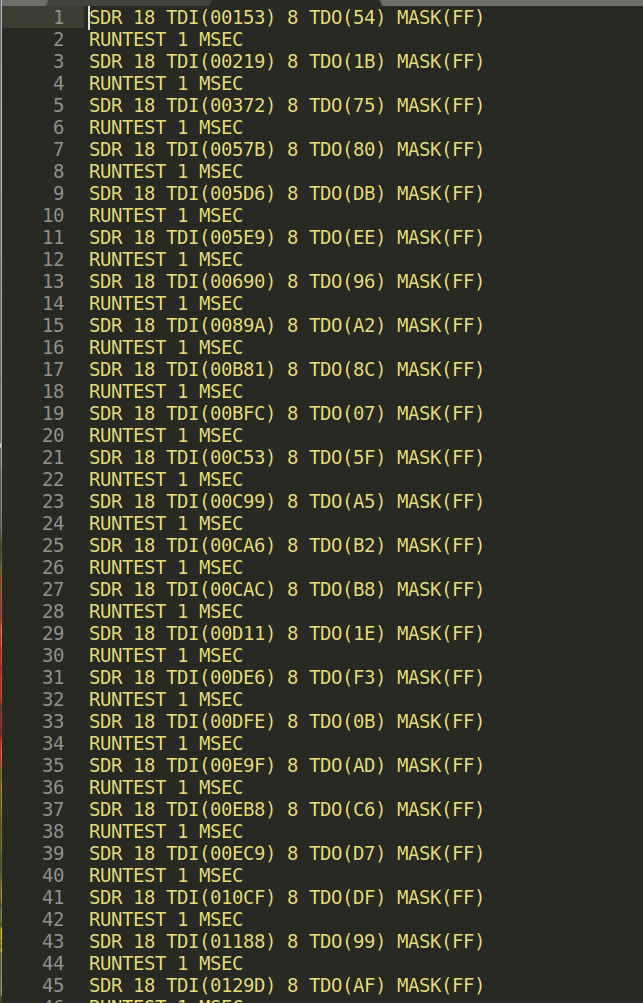
\includegraphics[width=70mm]{input.png}
                \caption{Truncated input}
            \end{subfigure}%
            \begin{subfigure}{.5\textwidth}
                \centering
                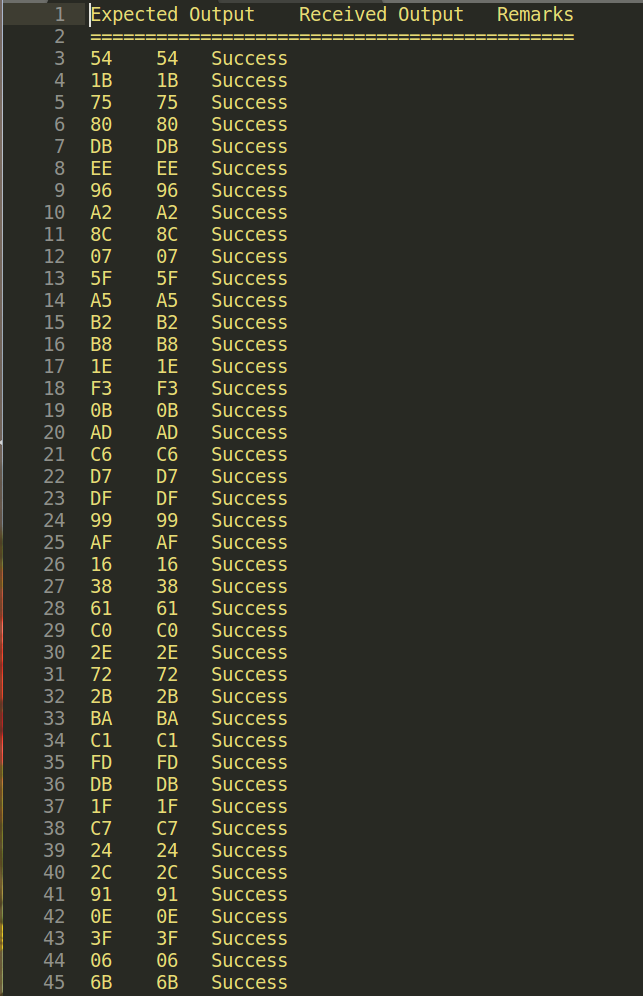
\includegraphics[width=70mm]{out.png}
                \caption{Truncated output}
            \end{subfigure}%
        \end{figure}

%%%%%%%%%%%%%%%%%%%%%%%%%%%%%%%%%%%%%%%%%%%%%%%%%%%%%%%%%%%%%%%%%%%%%%%%%%%%%%%%%%%%%%%%%%%%%%%%%%%%%
\newpage
\appendix
\section{Appendix}
    \subsection{Gates}
        \begin{minted}{vhdl}
library ieee;
use ieee.std_logic_1164.all;
package Gates is
  component INVERTER is
   port (A: in std_logic; Y: out std_logic);
  end component INVERTER;

  component welAND2 is
   port (A, B: in std_logic; Y: out std_logic);
  end component welAND2;

  component NAND2 is
   port (A, B: in std_logic; Y: out std_logic);
  end component NAND2;

  component welOR2 is
   port (A, B: in std_logic; Y: out std_logic);
  end component welOR2;

  component welNOR2 is
   port (A, B: in std_logic; Y: out std_logic);
  end component welNOR2;

  component welXOR2 is
   port (A, B: in std_logic; Y: out std_logic);
  end component welXOR2;

  component XNOR2 is
   port (A, B: in std_logic; Y: out std_logic);
  end component XNOR2;

  component HALF_ADDER is
   port (A, B: in std_logic; S, C: out std_logic);
  end component HALF_ADDER;

end package Gates;


library ieee;
use ieee.std_logic_1164.all;
entity INVERTER is
   port (A: in std_logic; Y: out std_logic);
end entity INVERTER;

architecture Equations of INVERTER is
begin
   Y <= not A;
end Equations;
  

library ieee;
use ieee.std_logic_1164.all;
entity welAND2 is
   port (A, B: in std_logic; Y: out std_logic);
end entity welAND2;

architecture Equations of welAND2 is
begin
   Y <= A and B;
end Equations;
  
library ieee;
use ieee.std_logic_1164.all;
entity NAND2 is
   port (A, B: in std_logic; Y: out std_logic);
end entity NAND2;

architecture Equations of NAND2 is
begin
   Y <= not (A and B);
end Equations;
  
library ieee;
use ieee.std_logic_1164.all;
entity welOR2 is
   port (A, B: in std_logic; Y: out std_logic);
end entity welOR2;

architecture Equations of welOR2 is
begin
   Y <= A or B;
end Equations;
  
library ieee;
use ieee.std_logic_1164.all;
entity welNOR2 is
   port (A, B: in std_logic; Y: out std_logic);
end entity welNOR2;

architecture Equations of welNOR2 is
begin
   Y <= not (A or B);
end Equations;
  

library ieee;
use ieee.std_logic_1164.all;
entity welXOR2 is
   port (A, B: in std_logic; Y: out std_logic);
end entity welXOR2;

architecture Equations of welXOR2 is
begin
   Y <= A xor B;
end Equations;
  
library ieee;
use ieee.std_logic_1164.all;
entity XNOR2 is
   port (A, B: in std_logic; Y: out std_logic);
end entity XNOR2;

architecture Equations of XNOR2 is
begin
   Y <= not (A xor B);
end Equations;
  
library ieee;
use ieee.std_logic_1164.all;
entity HALF_ADDER is
   port (A, B: in std_logic; S, C: out std_logic);
end entity HALF_ADDER;

architecture Equations of HALF_ADDER is
begin
   S <= (A xor B);
   C <= (A and B);
end Equations;
        \end{minted}
        
    \subsection{Tracefile}
    Below is the code for generating the required tracefile for testing of ALU:
    \begin{minted}{python}

f=open("./complete_ALU/TRACEFILE.txt","w") 

for x in range(256): 

    for y in range(256): 

        f.write("00{:08b}{:08b} {:08b} 11111111\n".format(x,y,(x+y)%256))

for x in range(256): 

    for y in range(256):

        f.write("01{:08b}{:08b} {:08b} 11111111\n".format(x,y,(x<<y)%256)) 

for x in range(256): 

    for y in range(256): 

        f.write("10{:08b}{:08b} {:08b} 11111111\n".format(x,y,(x>>y)%256)) 

for x in range(256): 

    for y in range(256): 

        f.write("11{:08b}{:08b} {:08b} 11111111\n".format(x,y,(x*y)%256)) 

f.close()     
    \end{minted}
    \vspace{5cm}
 $\ast$ For more references, check out my \textbf{github repo} on \href{https://github.com/v1an1/Codes-for-EE214-Digital-lab/tree/master/ALU}{\textbf{ALU}}\\
    

\end{document}
